\documentclass{article}


\usepackage{arxiv}

\usepackage[utf8]{inputenc} % allow utf-8 input
\usepackage[T1]{fontenc}    % use 8-bit T1 fonts
\usepackage{hyperref}       % hyperlinks
\usepackage{url}            % simple URL typesetting
\usepackage{booktabs}       % professional-quality tables
\usepackage{amsfonts}       % blackboard math symbols
\usepackage{nicefrac}       % compact symbols for 1/2, etc.
\usepackage{microtype}      % microtypography
\usepackage{lipsum}
\usepackage{graphicx}
\graphicspath{ {./images/} }

\author{
 Abud Santiago Elias \\
  Legajo 47015 \\
  \texttt{ sabudvicco@gmail.com} \\
   \And
 Castellano Marcelo \\
  Legajo 39028 \\
  \texttt{marce.geek22@gmail.com} \\
  \And
  Navarro Franco \\
  Legajo 46387 \\
  \texttt{franconavarro1889@gmail.com} \\
}


\title{TP 1.1 - SIMULACIÓN DE UNA RULETA}

\begin{document}
\maketitle
\begin{abstract}
  El trabajo de investigación a tratar en la siguiente documentación consiste en una simulación del funcionamiento de una ruleta, enfocándonos en técnicas probabilísticas y estadísticas para retratar lo más cercano a la realidad posible.

  Con los resultados obtenidos se busca retratar el comportamiento de la ruleta en la vida real sin tener en cuenta factores que en condiciones normales puedan afectar al número ganador.
\end{abstract}

% keywords can be removed
\keywords{ruleta \and simulación \and probabilidad \and estadística \and promedio \and números aleatorios \and azar}

\section{Introducción}
La ruleta es un juego de azar típico de los casinos, cuyo nombre viene del término francés roulette, que significa ``ruedita'' o ``rueda pequeña''. Su uso como elemento de juego de azar, aún en configuraciones distintas de la actual, no está documentado hasta bien entrada la Edad Media. Es de suponer que su referencia más antigua es la llamada Rueda de la Fortuna, de la que hay noticias a lo largo de toda la historia, prácticamente en todos los campos del saber humano.

La ``magia'' del movimiento de las ruedas tuvo que impactar a todas las generaciones. La aparente quietud del centro, el aumento de velocidad conforme nos alejamos de él, la posibilidad de que se detenga en un punto al azar; todo esto tuvo que influir en el desarrollo de distintos juegos que tienen la rueda como base.

Las ruedas, y por extensión las ruletas, siempre han tenido conexión con el mundo mágico y esotérico. Así, una de ellas forma parte del tarot, más precisamente de los que se conocen como arcanos mayores.

Según los indicios, la creación de una ruleta y sus normas de juego, muy similares a las que conocemos hoy en día, se debe a Blaise Pascal, matemático francés, quien ideó una ruleta con treinta y seis números (sin el cero), en la que se halla un extremado equilibrio en la posición en que está colocado cada número. La elección de 36 números da un alcance aún más vinculado a la magia (la suma de los primeros 36 números da el número mágico por excelencia: seiscientos sesenta y seis).

Esta ruleta podía usarse como entretenimiento en círculos de amistades. Sin embargo, a nivel de empresa que pone los medios y el personal para el entretenimiento de sus clientes, no era rentable, ya que estadísticamente todo lo que se apostaba se repartía en premios (probabilidad de 1/36 de acertar el número y ganar 36 veces lo apostado).

En 1842, los hermanos Blanc modificaron la ruleta añadiéndole un nuevo número, el 0, y la introdujeron inicialmente en el Casino de Montecarlo. Ésta es la ruleta que se conoce hoy en día, con una probabilidad de acertar de 1/37 y ganar 36 veces lo apostado, consiguiendo un margen para la casa del 2.7\% (1/37).

Más adelante, en algunas ruletas (sobre todo las que se usan en países anglosajones) se añadió un nuevo número (el doble cero), con lo cual el beneficio para el casino resultó ser doble (2/38 o 5.26\%).

\section{Marco teórico}
La ruleta es un clásico de los juegos de casino cuyo objetivo es predecir y acertar en qué casilla caerá la bola después de girar. Cuando el croupier así lo anuncie, el jugador deberá hacer apuestas en una o varias casillas de las 36 del tapete (sin contar el 0), justo antes de empezar la ronda.

El croupier lanzará la bola y cuando ésta deje de girar y se detenga en una de las casillas, quien hubiera apostado a esa casilla ganará un premio en función de su apuesta realizada.
La ruleta Montecarlo es la más conocida y la más extendida debido al origen francés del juego. Los números van del 0 al 36, y se juega con la regla de ‘en prisión’, una regla específica de la ruleta francesa. Según ésta, cuando sale el número 0, la mitad de las apuestas simples se devuelven a los apostantes, a diferencia de las otras modalidades donde el banco se queda todas las fichas. Gracias a esta regla y a que tiene 37 números (del 0 al 36 y un solo 0) es el tipo de ruleta que más beneficios ofrece para el jugador.

Lo más importante es tener claro que la ruleta es un juego de suerte y no de habilidad. Es cierto que el mismo número puede salir un par de veces en unos pocos giros, pero que esto suceda es pura casualidad, y es importante ver la ruleta como un juego de azar. Tanto si acaba de salir un número o si ya hace mucho tiempo que no sale, todos los números tienen las mismas probabilidades de que la bola se detenga en ellos. 

\subsection{Distribución uniforme discreta}
Función de probabilidad:
Se llama función de probabilidad de una variable aleatoria discreta X a la aplicación que asocia a cada valor de xi de la variable su probabilidad pi.
\begin{equation}
p_X(x_i) = P(X = x_i) = \frac{1}{n}
\end{equation}

Esperanza matemática:
También llamada valor esperado, es la sumatoria de las probabilidades de que exista un suceso aleatorio, multiplicado por el valor del suceso aleatorio.
\begin{equation}
\operatorname{E}[X] = \frac{a+b}{2}
\end{equation}

Varianza:
Es una medida de dispersión que representa la variabilidad de una serie de datos respecto a su media.
\begin{equation}
\operatorname{Var}(X) = \sigma^{2} = \frac{(b-a+1)^{2}-1}{12}
\end{equation}

Desvío estándar:
Es una medida que ofrece información sobre la dispersión media de una variable. La desviación estándar es siempre mayor o igual que cero.
\begin{equation}
\sigma = \sqrt{\operatorname{Var}(X)} = \sqrt{\frac{(b-a+1)^{2}-1}{12}}
\end{equation}

\subsection{Fórmulas muestrales}
Frecuencia relativa:
\begin{equation}
f_{i} = f_{r}(x_{i}) = \frac {n_{i}}{N}
\end{equation}

Esperanza matemática:
\begin{equation}
\operatorname{E}[X] = \sum_{i=1}^{n}x_{i}\,f_{i}=x_{1}f_{1}+x_{2}f_{2}+\cdots +x_{n}f_{n} = \frac{\sum_{i=1}^{n}x_{i}\,n_{i}}{N}
\end{equation}

Varianza:
\begin{equation}
\operatorname{Var}(X) = \sigma^{2} = \operatorname{E}\left[(X - \mu)^{2}\right] = \operatorname{E}\left[(X - \operatorname{E}[X])^{2}\right]
\end{equation}

Desvío estándar:
\begin{equation}
\sigma = \sqrt{\operatorname{Var}(X)} = \sqrt{\operatorname{E}\left[(X - \operatorname{E}[X])^{2}\right]}
\end{equation}

\section{Desarrollo}
La simulación del comportamiento se basa en una ruleta tipo Montecarlo, es decir,  los números están comprendidos del  0 al 36 (37 números en total).

En el presente estudio se utilizó un programa específico basado en el lenguaje de programación Python, el cual consistía en una carga de una lista con los números que aparecían conforme cada ronda fué sorteada. Los resultados obtenidos cada 100 rondas las denominamos como “Tirada” la cual nos permite tener una visión más global de los resultados y obtener los valores a los cuales tienden los resultados que se deseaban analizar.

A medida que avanzan las rondas se calcula la probabilidad, varianza y desvío estándar de cada una hasta que completa una tirada donde finalmente se calcula la esperanza matemática. Este proceso se repite durante 10 tiradas, cuyos números surgidos son guardados en una nueva lista global en la que se calculan los valores estadísticos mencionados nuevamente pero esta vez contando con una mayor muestra.

La finalidad de conocer estos resultados es analizar el comportamiento buscando tendencias o patrones que nos permitan en un futuro tratar de llegar a la elección de un  número dentro de un rango específico dados los resultados obtenidos.

%\pagebreak  % comenzar siguiente sección en una página aparte
\section{Resultados}
Como fué mencionado anteriormente se realiza el cálculo para saber los resultados del promedio, desvío y varianza de distintas tiradas de 100 rondas. A continuación se pueden ver las gráficas surgidas de cada una:

\begin{minipage}{0.5\textwidth}
  \begin{figure}[H]
  \centering
  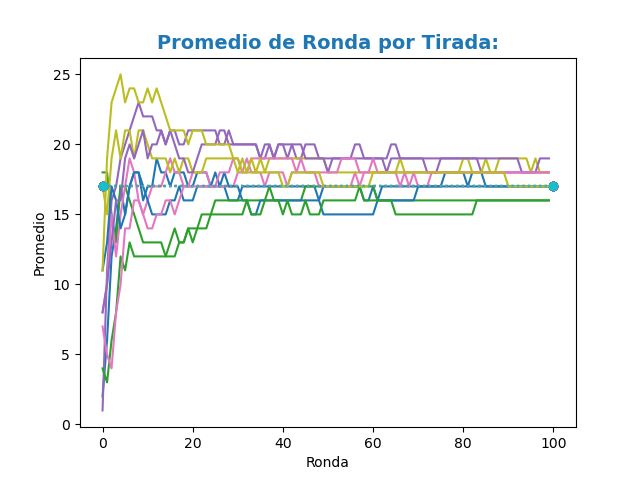
\includegraphics[width=\textwidth]{promedio-ronda-tirada.png}
  \caption{promedio calculado en cada ronda, graficado según su tirada}
  \label{fig:promedio-ronda-tirada}
  \end{figure}
\end{minipage}%
\begin{minipage}{0.5\textwidth}
Con el cálculo del promedio se trató de encontrar cual es el valor medio de los números aparecidos en cada ronda. En la gráfica podemos visualizar como el valor del promedio de cada tirada no se estabiliza si nó hasta la ronda 20 donde comienza a tomar valores más cercanos entre sí que rondan entre el 15 y el 20.
\end{minipage}

\begin{minipage}{0.5\textwidth}
  \begin{figure}[H]
  \centering
  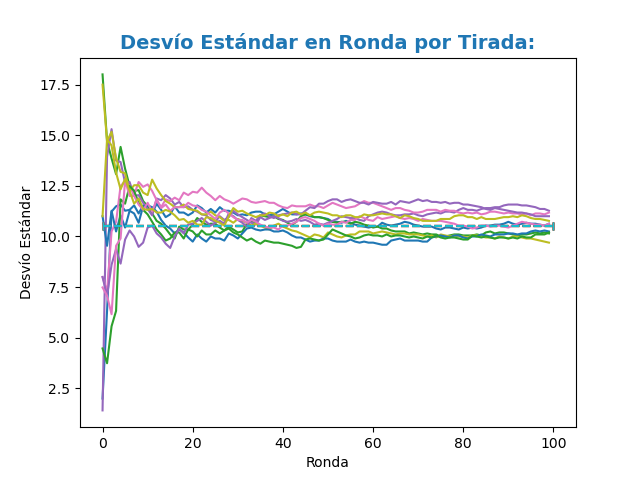
\includegraphics[width=\textwidth]{desvio-ronda-tirada.png}
  \caption{desvío estándar calculado en cada ronda graficada por tirada}
  \label{fig:desvio-ronda-tirada}
  \end{figure}
\end{minipage}%
\begin{minipage}{0.5\textwidth}
El fin de encontrar el desvío estándar en cada ronda es saber que tan alejado de la media se encuentra el número que surgió en la ronda, lo que nos permite saber cuánto dista un número surgido en una ronda con respecto al promedio. En la gráfica se puede ver que los valores de los resultados comienzan con distancias de hasta 17 unidades entre el número aparecido y la media. Hasta que aproximadamente en la ronda 20 comienza a tomar un valor más claro rondando entre el 10 y el 12 como se puede visualizar en la gráfica de cada tirada.
\end{minipage}

\begin{minipage}{0.5\textwidth}
  \begin{figure}[H]
  \centering
  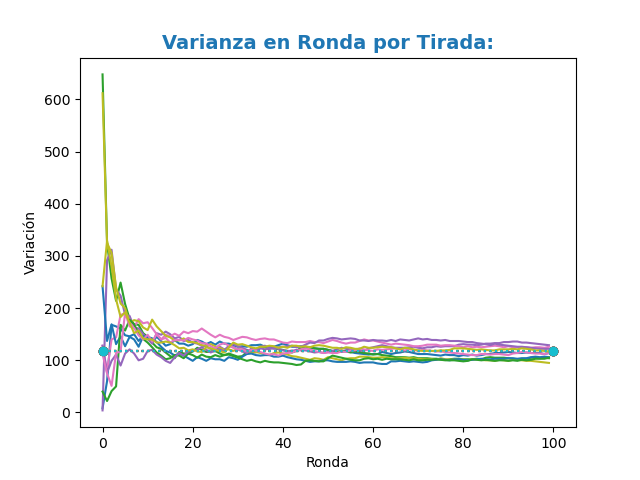
\includegraphics[width=\textwidth]{varianza-ronda-tirada.png}
  \caption{varianza calculada por ronda, graficada según su tirada}
  \label{fig:varianza-ronda-tirada}
  \end{figure}
\end{minipage}%
\begin{minipage}{0.5\textwidth}
Finalmente podemos visualizar la evolución de la varianza de cada tirada la cual sus valores rondan valores de entre 100 y 140.
\end{minipage}

A continuación se presentarán los resultados de la combinación de las 10 tiradas, lo cual representa un total de 1000 rondas, permitiendo tener una visión más exacta de los valores que se buscaban:
\begin{figure}[H]
  \centering
  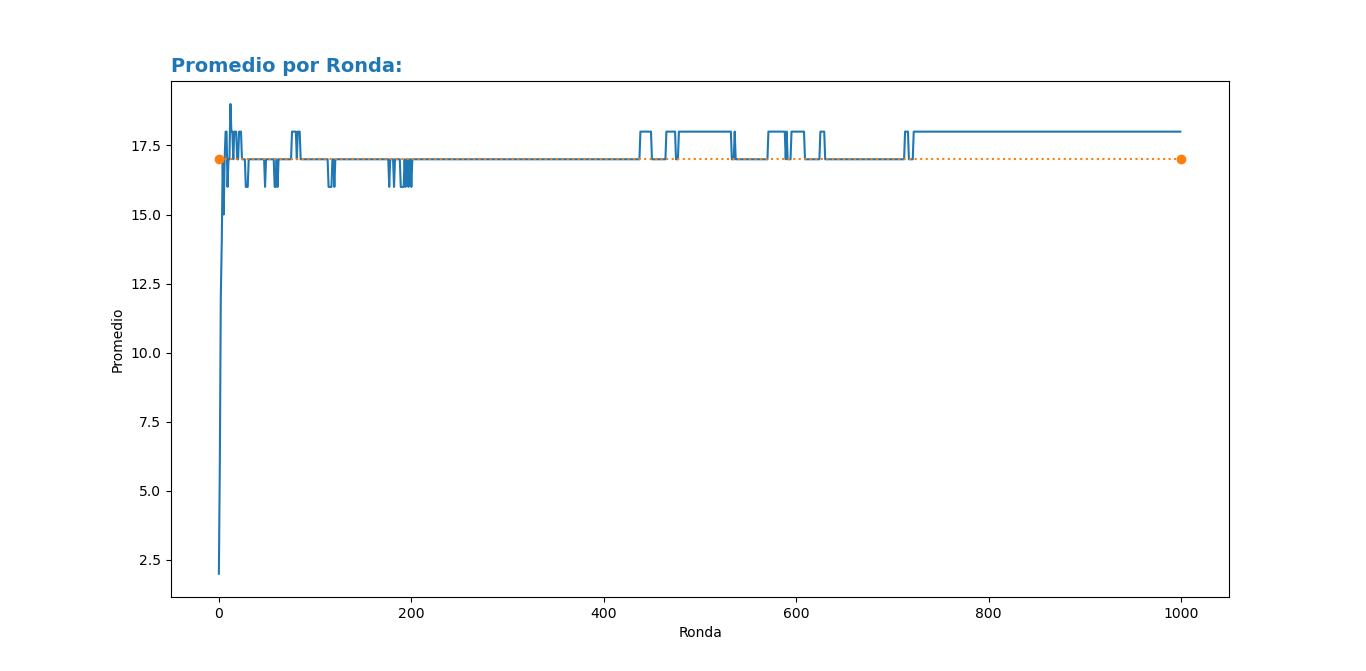
\includegraphics[width=0.5\textwidth]{promedio-ronda.png}
  \label{fig:promedio-ronda}
  \caption{promedio calculado por cada ronda}
\end{figure}
\begin{minipage}{0.5\textwidth}
  \begin{figure}[H]
    \centering
    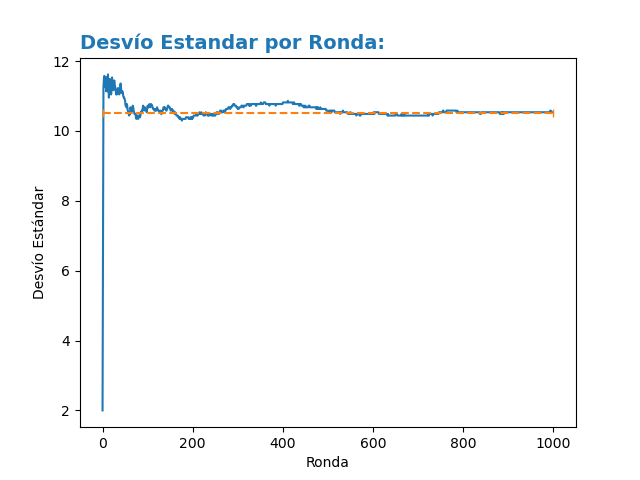
\includegraphics[width=\textwidth]{desvio-ronda.png}
    \label{fig:desvio-ronda}
    \caption{desvío estándar calculado por cada ronda}
  \end{figure}
\end{minipage}%
\begin{minipage}{0.5\textwidth}
  \begin{figure}[H]
    \centering
    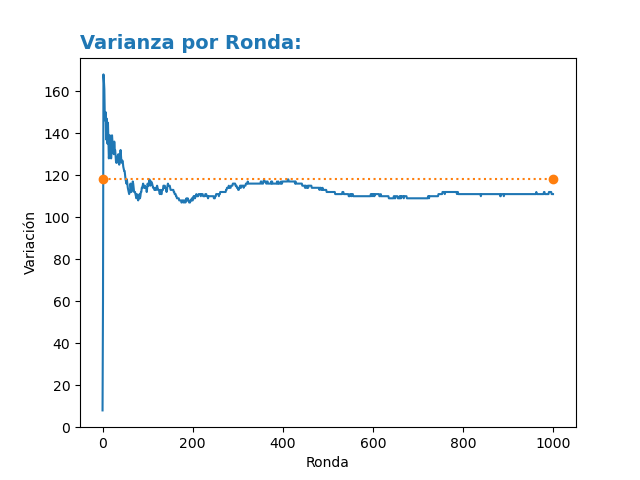
\includegraphics[width=\textwidth]{varianza-ronda.png}
    \label{fig:varianza-ronda}
    \caption{variación calculada por cada ronda}
  \end{figure}
\end{minipage}

Al realizar el cálculo de todos los valores en conjunto se puede visualizar como el valor esperado (línea de color naranja) se encuentra muy cercana a los valores que surgieron de los cálculos. Sin embargo esto es cierto para luego de una gran cantidad de rondas, ya que como vimos en las gráficas de las tiradas, los valores obtenidos no eran específicamente un número puntual, sino un rango de valores probables. Además de esto, llegar a estos números implica jugar 20 rondas.

Para finalizar se muestra una gráfica de dispersión, lo que pone en evidencia la aleatoriedad de los números y la frecuencia de aparición de cada número (según cada tirada).
\begin{figure}[H]
  \centering
  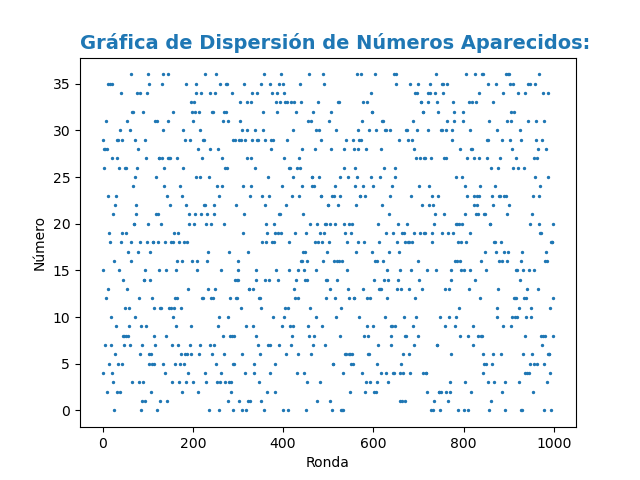
\includegraphics[width=0.5\textwidth]{dispersion.png}
  \label{fig:dispersion}
  \caption{gráfica de dispersión de los números aparecidos en cada ronda}
\end{figure}
\begin{figure}[H]
  \centering
  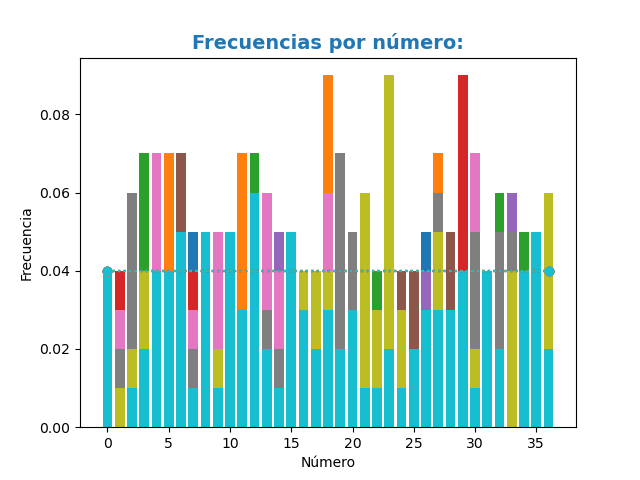
\includegraphics[width=0.4\textwidth]{frecuencias.png}
  \label{fig:frecuencias}
  \caption{frecuencia de aparición de cada número}
\end{figure}

\section{Conclusiones}
Como conclusión podemos afirmar que la simulación del funcionamiento de la ruleta fué exitosa debido a su aleatoriedad e inexistencia de tendencias en cuanto a un número o grupo de números específicos. Además, esto se puede confirmar viendo los resultados de los cálculos y las gráficas presentadas.

La utilización de la tecnología fue imprescindible para realizar la presente investigación debido a que sin ella sería casi imposible (o al menos muy largo y tedioso) realizar los cálculos presentados.

\nocite{*}  % citar toda la bibliografía
\bibliographystyle{unsrt}  
\bibliography{references}
\end{document}
